\section{Overview} \label{sec:design}
	\noindent For means of explanation, the architecture of the FPGA based implemented DRFM system can be described by three subsystems. These being, the interfacing and control system, the external peripherals and the DSP system. Whereby each of the constituent systems are monitored and controlled by the top-level controller module. This simplified architecture may be seen in Fig.~\ref{fig:DRFM_Architecture}.\\ \newline This being said, it must be noted that the architecture described in Fig.~\ref{fig:DRFM_Architecture} has not yet been integrated into a RF front end and therefore this paper is a review of the work in progress. The implications of this are that although real time signal processing and data storage are realizable at the speeds dictated by the RF front-end, it has not been shown that this architecture is in fact capable of achieving such speeds.
	\begin{figure*}[h!]
		\centering
		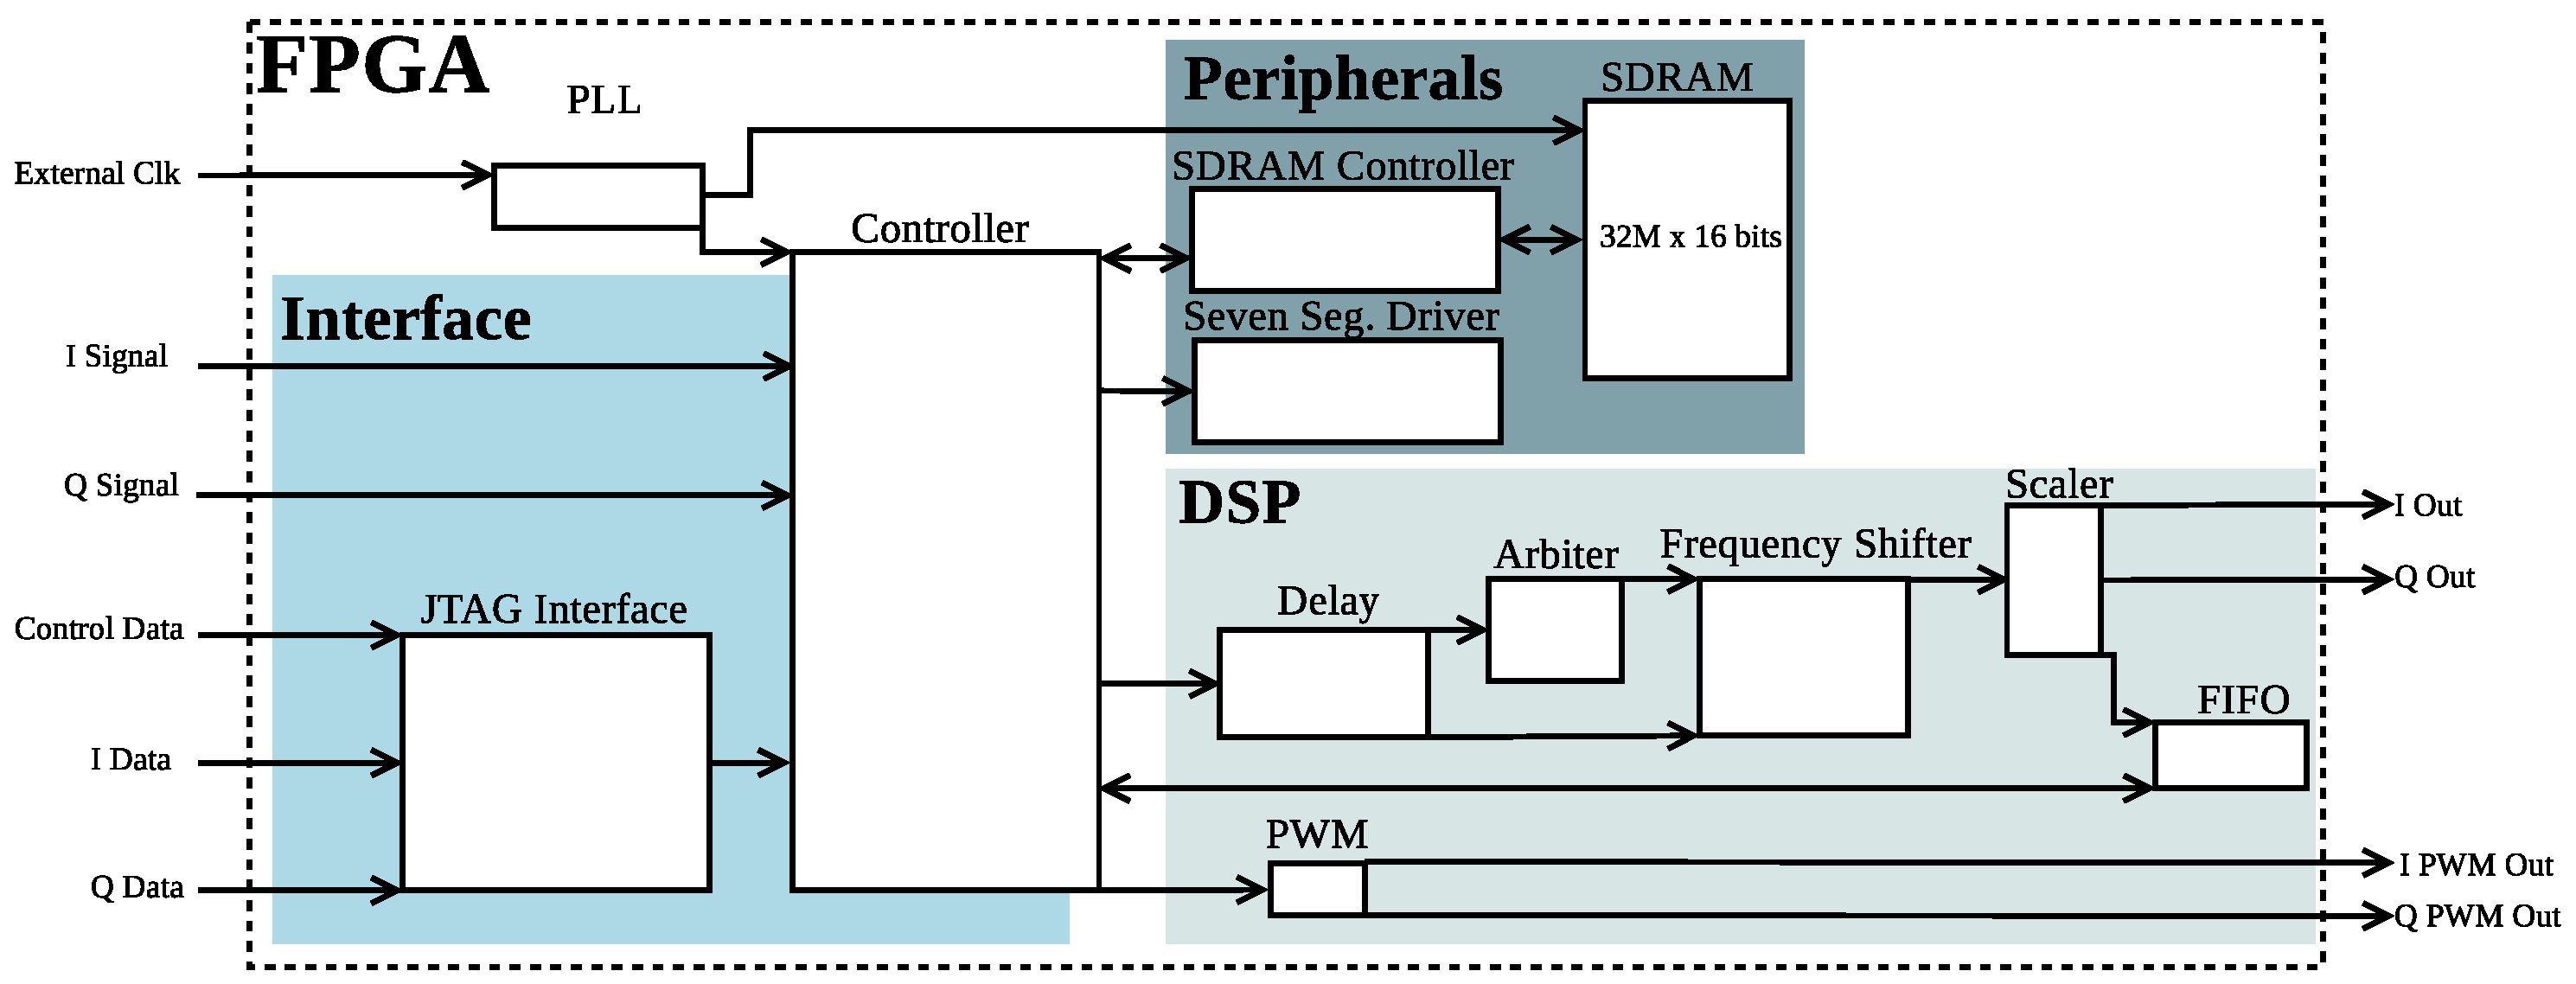
\includegraphics[width=0.95\linewidth]{img/System_Overview}
		\caption{Illustration of the implementation of the  FPGA based DRFM System}
		\label{fig:DRFM_Architecture}
	\end{figure*}
	
	\subsection{JTAG Interface}
		\noindent Joint Action Test Group (JTAG) was originally used as a simplified standard for interconnectivity testing for PCB manufacturing. It was created as a result of Integrated Circuits (IC) pins becoming more densely spaced and therefore classical interconnectivity test approaches were infeasible. The JTAG protocol mitigated the need for physical access to an IC's pins through the use of shift register chains.  \\ \newline In the JTAG standard (IEEE 1149.1) the collections of shift registers are referred to as Boundary Scan Cells (BSCs) which sample and hold data from and to the pin interface. As a result the BSCs can be configured into a serial shift chain thereby allowing to be driving by a serial interface. \\ \newline 	The JTAG interface implemented on the DRFM system allows for software based monitoring, updating and controlling of the DRFM system through the JTAG port.  Through the use of the Altera Virtual JTAG Intellectual Property (IP) core it is possible to access to the JTAG control signals that are routed to the FPGA core, which allow for a fine control over the JTAG resources thereby granting real-time general purpose serial communication \cite{JTAG}. \\ \newline	Through the use of  a Python based User Interface (UI) that runs a TCL JTAG server it is possible to direc
		
	
	\subsection{External Peripherals}
	
	\subsection{Signal Processing}
	
	\subsubsection{Time Delay}
	
	\subsubsection{Frequency shifting}
	
	\subsubsection{Fractional Amplitude Scaling}

	
	



